\documentclass[border=0pt]{standalone}
\usepackage{tikz}
\usetikzlibrary{decorations.markings, arrows.meta, positioning}

\definecolor{curvegreen}{RGB}{26, 143, 63}
\definecolor{lineyellow}{RGB}{236, 168, 25}

\begin{document}
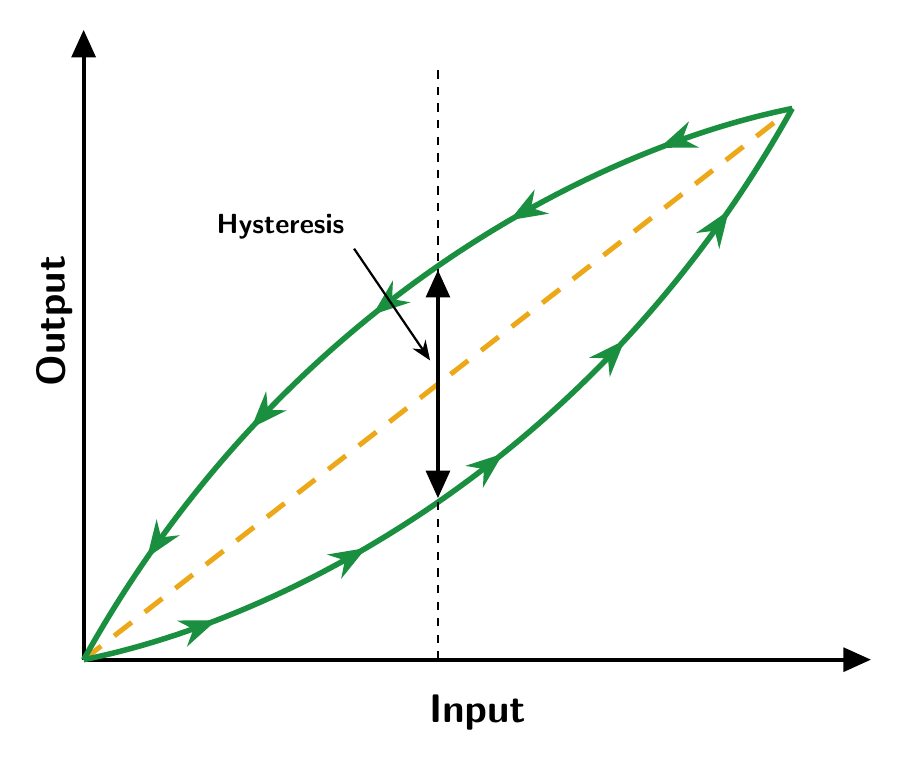
\begin{tikzpicture}[
    >={Triangle[length=3.5mm, width=3mm]},
    curve arrow/.style={
        decoration={
            markings,
            mark=between positions 0.15 and 0.9 step 0.18 with {\arrow[scale=1.1, curvegreen]{Stealth}}
        },
        postaction={decorate}
    }
]

% Axes
\draw[->, line width=1.5pt] (0,0) -- (10,0) node[midway, below=0.3cm, font=\sffamily\Large\bfseries] {Input};
\draw[->, line width=1.5pt] (0,0) -- (0,8) node[midway, above=0.3cm, rotate=90, font=\sffamily\Large\bfseries] {Output};

% Dashed center line
\draw[line width=1.8pt, dashed, lineyellow, dash pattern=on 8pt off 6pt] (0,0) -- (9,7);

% Lower curve (Forward/Up)
\draw[line width=2pt, curvegreen, curve arrow] 
    (0,0) .. controls (2.5, 0.5) and (6.5, 2.5) .. (9,7);

% Upper curve (Backward/Down)
\draw[line width=2pt, curvegreen, curve arrow] 
    (9,7) .. controls (6.5, 6.5) and (2.5, 4.5) .. (0,0);

% Vertical dashed line
\draw[dashed, thick] (4.5, 0) -- (4.5, 7.5);

% Double headed arrow for Hysteresis gap
\draw[<->, line width=1.5pt] (4.5, 2.05) -- (4.5, 4.95);

% Annotation
\node[font=\sffamily\bfseries] (HystLabel) at (2.5, 5.5) {Hysteresis};
\draw[-{Stealth[length=2.5mm, width=2mm]}, thick] (HystLabel.south east) -- (4.4, 3.8);

\end{tikzpicture}
\end{document}